\documentclass[12pt]{article}\usepackage[]{graphicx}\usepackage[]{color}
% maxwidth is the original width if it is less than linewidth
% otherwise use linewidth (to make sure the graphics do not exceed the margin)
\makeatletter
\def\maxwidth{ %
  \ifdim\Gin@nat@width>\linewidth
    \linewidth
  \else
    \Gin@nat@width
  \fi
}
\makeatother

\definecolor{fgcolor}{rgb}{0.345, 0.345, 0.345}
\newcommand{\hlnum}[1]{\textcolor[rgb]{0.686,0.059,0.569}{#1}}%
\newcommand{\hlstr}[1]{\textcolor[rgb]{0.192,0.494,0.8}{#1}}%
\newcommand{\hlcom}[1]{\textcolor[rgb]{0.678,0.584,0.686}{\textit{#1}}}%
\newcommand{\hlopt}[1]{\textcolor[rgb]{0,0,0}{#1}}%
\newcommand{\hlstd}[1]{\textcolor[rgb]{0.345,0.345,0.345}{#1}}%
\newcommand{\hlkwa}[1]{\textcolor[rgb]{0.161,0.373,0.58}{\textbf{#1}}}%
\newcommand{\hlkwb}[1]{\textcolor[rgb]{0.69,0.353,0.396}{#1}}%
\newcommand{\hlkwc}[1]{\textcolor[rgb]{0.333,0.667,0.333}{#1}}%
\newcommand{\hlkwd}[1]{\textcolor[rgb]{0.737,0.353,0.396}{\textbf{#1}}}%
\let\hlipl\hlkwb

\usepackage{framed}
\makeatletter
\newenvironment{kframe}{%
 \def\at@end@of@kframe{}%
 \ifinner\ifhmode%
  \def\at@end@of@kframe{\end{minipage}}%
  \begin{minipage}{\columnwidth}%
 \fi\fi%
 \def\FrameCommand##1{\hskip\@totalleftmargin \hskip-\fboxsep
 \colorbox{shadecolor}{##1}\hskip-\fboxsep
     % There is no \\@totalrightmargin, so:
     \hskip-\linewidth \hskip-\@totalleftmargin \hskip\columnwidth}%
 \MakeFramed {\advance\hsize-\width
   \@totalleftmargin\z@ \linewidth\hsize
   \@setminipage}}%
 {\par\unskip\endMakeFramed%
 \at@end@of@kframe}
\makeatother

\definecolor{shadecolor}{rgb}{.97, .97, .97}
\definecolor{messagecolor}{rgb}{0, 0, 0}
\definecolor{warningcolor}{rgb}{1, 0, 1}
\definecolor{errorcolor}{rgb}{1, 0, 0}
\newenvironment{knitrout}{}{} % an empty environment to be redefined in TeX

\usepackage{alltt}
\usepackage[top=1.00in, bottom=1.0in, left=1.1in, right=1.1in]{geometry}
\renewcommand{\baselinestretch}{1.1}
\usepackage{graphicx}
\usepackage{natbib}
\usepackage{amsmath}
\bibliographystyle{..//refs/styles/besjournals.bst}
\def\labelitemi{--}
\parindent=24pt


\title{Reconciling historic hypotheses regarding flower-leaf sequences in temperate forests for fundamental and global change biology}
% Alt: Re-ordering phenology: Reconciling historic hypotheses regarding flower-leaf sequences with their high variability
% Alt: Why many species flower before they leaf in temperate forests and how climate change may reshape phenological sequences
% Alt: Reconciling historic hypotheses regarding flower-leaf sequences in temperate forests for fundamental and global change biology
%old A series of phenological events: Reconciling historic hypotheses regarding flower-leaf sequences in temperate forests
\author{Daniel Buonaiuto, Nacho, Lizzie}
\date{July 28, 2019}
\IfFileExists{upquote.sty}{\usepackage{upquote}}{}
\begin{document}

\maketitle
To Do:
\begin{enumerate}
\end{enumerate}
\section*{Abstract}

\indent\indent As the study of phenology progresses as a discipline, it is increasing clear that it is not only individual phenological events that affect organism fitness and ecological functioning, but also the relationship between stages.  Deciduous woody plant species exhibit remarkable varaition in flower-leaf  sequence's (FLS's), or the relative order of their spring reproductive and vegetative phenolgoical events. A century of research suggests that FLS patterns are adaptive, and several competing hypotheses stand to explain their evolution and function. \\
\indent But reconciling these hypotheses has been impeded by our conceptual framework for understanding these patterns. Classically, FLS's are treated as discrete catagories and described at the species level. However, long-term phenological data suggest there is considerable intra-specific variation in FLS's that is unaddressed in the current hypotheses, and that FLS catagorization further obscures interspecific differences.
% Try to make the below more exciting, I did a little below but more needed.
Here, we review and modify the existing hypotheses to account for the high levels of intra-specific FLS variation seen in nature. We then evaluate these hypotheses with four case studies from temperature forest species.\\ 
 \indent Our review and case studies provide three major insights towards a new conceptual framework for understanding FLS. First, we find support for multiple hypotheses. Future research should accomidate this coincidence both by allowing for overlapping hypotheses in large community models and by testing individual hypotheses in smaller sub-groupings that control for variation in other traits. % This last sentence is great! Make sure the reader gets this point in your discussion!
Second, we show that the support for FLS hypotheses is highly sensitive to how FLS's are defined. Researchers should, when possible, move away from the classic categorization scheme of FLS and use standarized, continuous measures of FLS. Finally, researchers should use these intra-specific, continuous measures of FLS to test for fitness consequences in FLS variation. This will advance our understanding of the fundamental biology of FLS patterns, and help us to predict how climate related alterations to FLS's will affect tree communities in the changing future.

% ...to reduce the impact of observer bias, and allow for stronger inference regarding FLS variability among and within species
%Am nat 200 words
%250 AJB
%350 JoE
%currently 305


\section*{Introduction}
% Good stuff here in the first couple paragraphs
\indent \indent Phenology, the timing of seasonal life cycle events, allows organisms to synchronize important life history transitions with optimum environmental conditions \citep{Forrest2010}, and is a critical component of ecosystem structure and function \citep{Cleland2007,Piao2007}. Recent work in woody plant phenology has shown that it is not only individual phenological stages that affect these processes, but also the relationship between them \citep{Ettinger2018}.\\
\indent One phenological relationship that has long received scientific interest (see \citet{Robertson1895}), and recently, increased attention in the literature is the flower-leaf phenological sequence (FLS) of decidiuous woody plants. In a typical model of plant life history, vegetative growth precedes reproduction. However, for many species in the forests of Eastern North America, it is not the green tips of new shoots that mark the commencement of the growing season, but the subtle, reds, and yellows of their flowers. This flowering-first FLS is common in these regions, and its prevalence suggests that this FLS has adaptive significance \citep{Rathcke_1985}.\\ 
\indent A deep inquiry into the nature of this phenological pattern is necessary and timely because anthropogenic climate change is altering FLS's (Fig. \ref{fig:Figure 1}). For the three European tree species we examined, the number of days between flowering and leafout have increased as a result of climate change, but the rate of change differs amoung them. %For one species, (\textit{Fraxinus excelsior}), the time between flowering and leafout has already increased beyond its historic range of variability, while the others show more muted responses.
If, as suggested, optimum FLS timing is an important componenet of fitness, this differential FLS sensitivity to climate change may influence which species can adapt to new climate conditions and persist into the future.\\
% Explain in a sentence with example or such why you might get a change? DB cues?
\indent Despite recent advances in characterizing the evolution and underlying physiology of FLS \citep{Gougherty2018,Savage2019}, a major challenge to predicting how FLS patterns will shift in response to climate change is that we don't have a very good baseline understanding of variability in FLS.
% Some changes to how we reference the figures ... needs work on language though -- can you just say it simply: days between X and Y are increasing/decreasing
% Also, can you add a little foreshadowing here about intraspecific variation?
While some authors present general correlations between flowering and leafing phenology \citep{Lechowicz_1995, Ettinger2018}, fine scale FLS variability has never been evaluated. We suggest that characterizing FLS variation among individuals and populations will not only improve our ability to predict how FLS patterns will change in the future, but also allow for a more biologically relevant evaluation of the current FLS hypotheses and reveal avenues for future, direct hypothesis testing.\\
\indent Here we 1) Review the adaptive hypotheses of FLS and their respective predictions, 2) Evaluate variation in FLS, and explore how FLS variation within species, populations and individuals alters the predictions of the hypotheses, 3) Show how the incorporation of variation alters which hypotheses are supported using case studies from temperate forests, and 4) make recommendations for future study of FLS. 
\section*{Defining FLS}
\indent\indent Flower-leaf sequences have traditionally been classified into distinct qualitative categories that are almost always defined at the species level. The terms hysteranthy, protanthy, proteranthy or precocious flowering describe plants that produce flowers before their leaves \citep{Lamont2011, Heinig1899}. A classic example of this FLS is \textit{Acer rubrum}, which, as seen in figure \ref{fig:Figure 2}, reaches peak flowering weeks before any sign of leave development. These species tend to exhibit a degree of physiological specialization, such as the separation of flower and leaf buds. \\
\indent Seranthy %\ref{fig:Figure 2} \textit{Nyssa sylvatica}, 
describes species in which flowers open as leaves approach their full size. These species can still differentiate flower buds in the previous season, but may rely less on stored energy than flowering-first taxa.\\
\indent But what about species whose FLS separation is less clear? It is possible to describe all species whose flowering period overlaps their leaf development as synanthous \citep{Lamont2011}, but this third category may obscure important inter-specific differences.\\ %Furthermore, both the flowering and leaf growth periods consist of several sub-stages making it difficult to fit FLS patterns neatly into these categories.\\
 \indent Take \textit{Betula alleghaniensis} from figure \ref{fig:Figure 2} for example: One would be justified in classifying this species as hysteranthous because its flower buds tend to burst before its leaf buds, or as synanthous because its open flowers overlap the beginning of leaf growth. Can we really put this species in the same category as \textit{Acer rubrum}, whose flowers open weeks before the leaves? Conversely, is this species truly more similar to figure \ref{fig:Figure 2}'s \textit{Acer pensylvanicum} whose flowers do not open until leaves are well along in their expansion? \\
\indent  The FLS classification scheme relies on the judement of each individual observer making it difficult to synthesize information across datasets. If a species is called hysteranthous in one dataset and synanthous in another, should we interpret this as temporal or geographic variability in FLS or an artifact of observer decision-making? This uncertainty hampers our ability to accurately test the exisiting FLS hypotheses, because any statistical relationship between FLS and other traits is biased by the classifier. However, a way forward through this bias is possible by examining the biological mechanisms underdlying each hypotheses and incoprerating the predictions they make regarding FLS overlap and variability in to analyses.
 
\section*{Hypotheses of FLS and their predictions about flower-leaf overlap}
\indent \indent Each prevailing FLS hypothesis suggests evolutionary drivers that produce the phenological sequences observed today. These mechansims accomidate a different degree of overlap between vegetative and floral phenophases. Here, we review the current FLS hypotheses, identify the underlying biology of each, and make predictions about how much phenological overlap between flowering and vegtative growth they can accomidate.

\subsubsection*{ Wind pollination}
\indent\indent The most prevalent FLS hypothesis associates hysteranthous flowering with pollination syndrome, suggesting that hysteranthy is an adaptation critical for effective wind pollination, with leafless flowering allowing for more efficient pollen dispersal and transfer \citep{Whitehead1969, Spurr1980,Friedman2009}. %In support of this hypothesis, it has been shown that wind velocities in forests are considerably higher in the leafless season than when a canopy is full \citep*{Brown1969,Whitehead1969}. and that vegetation structure and canopy closure reduce particle diffusion through a forest\citep{Brown1969}. Other studies have shown that there is significant filtration of pollen by leaves \citep*{Milleron2012, Tauber1967}, with the amount of pollen impacted on non-floral structure increasing by ~400\% between the leafless season and canopy expansion \citep{Tauber1967}.\\
 This hypothesis hinges on the fact that leaves create a substantial physical disruption to pollen transfer, a premise that we would not necessarily expect to be true for the early stages of leaf expansion when tiny leaf primordia would have little impact on environmental structure. In this framework, we expect that trees that flower during the early stages of leaf expansion would gain similar mechanical advantage to those who complete their flowering before any leaf activity, and we see evidence for this in the phenological records from Harvard Forest. While wind-pollinated species flower both before and after bud burst, the flowering of all species takes place before their leaves reach 75\% of their final size. This hypothesis predicts that wind pollinated species should flower before or with their leaves, while in animal pollinated species, FLS should be random or co-vary with pollinator activities.
\subsubsection*{Water dynamics}
\indent\indent Another hysteranthous hypothesis, emerging from the dry deciduous tropics where flowering during the leafless season is also common \citep{Janzen1967}, suggests that flowering before leaf development is an adaptation to reduce water stress associated with maintaining floral hydration while leaves are transpiring \citep{Franklin2016}. %While this hypothesis has been primarily discussed for dry tropical flora, recent work has linked flowering-first FLS to drought tolerance in temperate flora as well \citep{Gougherty2018}.\\
This hypothesis asserts a significant cost to maintaining floral structures during any stage of leaf activity, and therefore only species whose flowering occurred before any leaf expansion would gain this drought advantage. This hypothesis predicts that species that are drought tolerant should flower before leafing out, with minimal overlap between the floral and vegetative phenophases. Species that are not drought tolerant gain no real advantage from flowering first, so in these species FLS should be random. %%or is it less about drought tolerance and more about living in dry environments. Are these different?
\subsubsection*{Early flowering}
\indent\indent A third possibility is flowering-first FLS is a physiological byproduct of selection for early flowering \citep{Primack1987}. % Authors have associated flowering-first FLS with functional traits such as seed mass and development time , cold tolerance \citep{}, and wood anatomy \citep{}, all traits that have been suggested as evolutionary drivers of early phenological activity.
Within this framework, there is no advantage to a species being hysteranthous vs. seranthous, as long as the absolute flowering time of the contrasting FLS's were the same. %However, this equivalency may be a physiological impossibility. 
However, recent work from \citet{Savage2019} has demonstrated that floral hydration is independent of the xylem and primarily maintained by the phloem. With leaf phenology constrained by the timing xylem re-genisis, selection for early season reproduction drives flowering into the early season when xylem function is still supressed, producting the hysteranthous FLS. This might explain why hysteranthous species tend to be the earliest species to flower. Here, we expect the increased time between flowering and leaf out to be associated with earlier flowering phenology in general. We expect to see strong associations with other early flowering traits such as seed mass, dispersal season or cold tolerance. However, this hypothesis does not require the selective driver of early flowering to be exclusively one of these traits, and pollination syndrome or drought tolerance may still play a role in driving the early flowering \citep{Savage2019}.\\
\indent This hypothesis predicts that species' flowering times should be strongly associate with flowering-first FLS. It also is likely there would be relationship between this FLS and other early flowering traits.
\subsubsection*{Phylogenetics} 
\indent\indent Finally, it is also possible that FLS's are highly conserved traits, and the preponderance of hysteranthy in the temperate zone is a product of phylogenetic representation of the region rather than an adaptive quality to the trait. In this framework, FLS is under very weak or no selection so there are no expectations regarding the degree over overlap between flower and leaf phenological activity, only that FLS's should map well onto a phylogeny.  
This hypothesis predicts strong phylogenetic patterning in the FLS with no correlation a priori expected with other traits.\\
%\indent  Of course, none of these hypotheses are mutually exclusive. It is is certainly possible that FLS has arisen multiple times in different evolutionary environments, and remnants of all these selective forces may be present in temperate eastern forest taxa, maintained by the strong seasonality of the region and land standing evolutionary trade offs. 
% Add a short conclusions section hereon why figuring out these hypotheses NOW is most important for fundamental science, and for climate change, which has made this variation more obvious ... transition to variation. 
\section*{Variation in FLS}
 \indent\indent All of the above hypotheses assume that FLS's are a species-level trait, however, this assumption has not been well examined in the literature \citep[e.g.,][]{Gougherty2018}. Intra-specific variation is the engine of natural selection, and if it is substantial in FLS patterns, we can infer much about origins of this trait, and its trajectory as the climate changes.
 We investigated individual FLS variation using a long term phenological data set collected at Harvard Forest in Petersham, Massachusetts \citep{OKeefe2015}. The time between flowering and leaf activity varied by as much as several weeks for most species.  This variability  can significantly blur FLS categorization. For example,  \textit{Q. rubra}), a species classically listed as flowering and leafing in synanthy, there are some years in which flower budburst is over a week before leaf budburst, and other years, in which leaf buds burst weeks prior to floral budburst (Fig. \ref{fig: Figure 3}). We also found significant population level variation in FLS, using the Pan European phenological database PEP725 \citep{PEP725}, with the average time between flowering and leafing varying between sites by a week more.\\
\indent Given the variability of FLS at the individual and population level, it is clear that considering FLS variability at only higher taxonomic levels may obscure important realities about the biology of this phenological trait. Below, we discuss how the observed variation below the species level may alter the existing FLS hypotheses.

\subsection*{How FLS variation alters predictions}
\subsubsection*{Wind pollination} 
\indent\indent  Pollination syndrome is generally treated as a species level trait, considered to be fairly immutable across ecological time and space. Because of this, we would not expect significant variation in FLS across population or individuals because we would not expect variation in pollination syndrome. However, as discussed above, a tree with no overlap between flowering and leafing phenology does not necessarily gain a significant pollen transfer advantage over an individual with some overlap. The pollination efficiency advantage from flowering-first diminishes as the canopy fills in, but  we do not know at what point during leaf expansion pollination would become significantly encumbered. It is possible that interannual and population level variation in hysteranthous FLS could maintain a wind pollination advantage, as long as the overlap did not cross a certain unknown threshold. Therefore, based on the wind pollination efficiency hypothesis, we would not expect high levels of population or individual variation in FLS, but the detection of some FLS variability at these levels, does not inherently challenge the plausibility of the hypothesis.
\subsubsection*{Water dynamics} 
\indent\indent If FLS's are driven by water dynamics, we would expect there to be significant population level variation in FLS. Populations growing in drier habitats should show flower earlier relative to their leaf activity than their counterparts growing in wetter areas with more relaxed selection on minimizing phenological overlap. Therefore, increased time between flowering and leafing should be negativly correlated with average soil moisture. Water availability may also drive interannual FLS variation, with drought years increasing hysteranthy, and wetter years permitting more FLS overlap. Because plants have many other physiological mechanisms for dealing with occasional drought, we only expect to see a signal for the association between a drought tolerance and hysteranthy for observations of populations in drought prone regions. 
\subsubsection*{Early flowering} 
\indent\indent This hypothesis predicts some variation on the population level based on local adaptation.  We would expect populations in which selection for earlier phenology is stronger, perhaps those in regions with shorter growing seasons, to show a higher degree of hysteranthy.  At the individual level, FLS variability could be driven by interannual variability in spring conditions. Both flowering and leaf phenology are strongly cued to temperature and photoperiod \citep{Flynn2018,Rathcke_1985}, but with leaf phenology constrained by xylem activity and flowering phenology relatively independent of it, we would expect a stronger response to environment in flowering time resulting in FLS variation.  Below the species level, this hypothesis predicts that early flowering years or populations are associated with increased time between flowering and leafing for hysteranthous species.
\subsubsection*{Phylogenetics} 
\indent\indent With the lack of treatment of FLS variability in the literature below the species level, we have no strong basis for asserting whether the apparent variability in FLS is a product of genetic or environmental controls. If there is a strong genetic component to FLS as has been show in other phenophases \citep{Wilczek2010}, some population level variation could be driven by reproductive isolation. With strong genetic control of FLS, we might also see consistent genotypic differences in FLS among individuals within a population, but would not predict high levels of interannual variation.\\
%%do we need to talk about predictions for seranthy anywhere

%\indent There is substantial variation in FLS as the population and individual levels. When considering the FLS hypotheses in the context of this variation, some of them, predict that there should be less variation. Just as at the species level, the exact predictions of these hypothesis operating withing species rely on how one chooses to demarcate FLS patterns in relation to overlap between floral and foliate phenophases. 

\section*{Available evidence for FLS hypotheses in temperate woody species} 
\indent\indent Despite a strong conceptual basis, direct tests of these hypotheses of hysteranthy in the literature are relatively rare, and--when tested---support for them is mixed. Many studies only test a single hypothesis, making comparison between them difficult. For example, the primary evidence supporting the wind pollination hypotheses comes from pollen diffusion studies, e.g., particle movement through closed and open canopies \citep{Niklas1985,Nathan2005, Milleron2012}, which provide no framework for comparatively evaluating the other hysteranthy hypotheses. We are aware of no direct test that have tried and distinguish selection for hysteranthy from selection for early flowering, but \citet{Primack1987} notes that hysteranthous, wind-pollinated species tend to also have large seed mass, and lack primary seed dormancy for germination, traits associated with early flowering in general. This raises the distinct possibility that hysteranthy may simply be one component of a larger suit of early flowering traits. We are also aware of no studies that have mechanistically evaluated the water dynamics hypothesis, though observations of flowering in the dry tropics by \citet{Borchert1983,Reich1984} suggest that the timing of flowering in hysteranthous taxa is associated with a plant water status recovery due to leaf drop. Only recently has it even been suggested that this hypothesis might be relevant in the temperate zone as well, as it is not expected that water status would limit biological activity in the wet spring months of the temperate zone \citep{Gougherty2018}.\\
\indent In contrast, studies testing multiple hypotheses have generally found support for more than one evolutionary driver of hysteranthy. One study by \citet{Bolmgren2003} showed that wind pollinated species tend to also be earlier flowering than their biotocially pollinated sister taxa, suggesting a relationship between the early flowering and wind pollination hypotheses. A recent study by \citet{Gougherty2018} tested multiple hypotheses by modeling associations between species' trait and FLS patterns in the Great Lakes regions. They found strong support for both the water dynamics and early flowering (flower timing and seed characteristics) hypotheses, and found strong phylogenetic clustering for FLS. \\
\indent In all of these cases, variability in FLS below the species level was not addressed. Yet, there are datasets widely available that would allow for testing these several hysteranthy hypotheses concurrently, and at multiple taxonomic levels. To address this gap, we supplement our literature review by re-testing some previously-used datasets to examine all hypotheses, and we leverage several widely-available datasets to test how support for these hypotheses varies across the inter- to intra-specific levels.\\ 
\indent We evaluated hysteranthy in four phenological datasets. Michigan Trees and its companion volume Michigan Shrubs and Vines \citep{Barnes2004,Barnes2016} (MTSV) contains categorical FLS information for 195 woody plant species. The USFS Silvics manual volume II \citep{Burns1990} contains categorical FLS descriptions for 81 woody species. These data can be used to test inter-specific FLS variation. Within these datasets, we applied two alternative FLS classification schemes; physiological hysteranthy, which allowed for no overlap between floral and leaf phenophases, and functional hysteranthy, which allowed for a degree of overlap as predicted by the wind pollination hypotheses. The Harvard Forest dataset (HF) contains quantitative flowering and leaf phenology measurements for individuals of 24 woody species over a 15 year period, allowing for both inter- and intra-specific comparisons \citep{OKeefe2015}. In this data set, we approximated the two hysteranthy classification schemes mentioned above by measuring the temporal offset between different floral and leaf phenophases. From the Pan European Phenological Database (PEP725) \citep{PEP725} we obtained spatially and temporally explicit, quantitative flowering and leaf phenology for four common European tree species. This allows for the evaluation of FLS only at the intra-specific level, but unlike the other datasets, it allows for population level variability to be assessed.\\
\indent In considering each species-level data set separately and in tandem two clear trend emerge: One, in accordance with the recent literature, we found support for multiple hypotheses. There was generally strong support for the early flowering and wind pollination hypotheses, poor support for the water dynamics hypothesis, and the phylogenetic signal was variable (figure \ref{fig:Figure S1}). The support for multiple hypotheses is not terribly surprising. We wouldn't expect the wind pollination hypothesis to explain hysteranthy in biotically pollinated taxa. Further, given the almost constant non-equilibrium state of temperate forest communities due to glacial cycles over the last 10,000 years \citep{Spurr1980}, it is not surprising our flora consists of species with radically different bio-geographic histories that may have evolved hysteranthous flower under very different selection environments. \\
% Below is important and should be start of a paragraph ... or new section!
\indent The second clear signature from our analysis was that relative importance of each the predictors changed significantly depending on how hysteranthy was defined. Generally, this artifact was minimized when continuous measure of FLS were used over categorical.\\
% Below is  too long and unfocused, can you break into multiple paragraphs with clear points? I almost entirely missed anything about quantitative versus categorical ... 
\indent When considering our intra-specific datasets, contrary to what we predicted given the water dynamics hypothesis, intra-annual variation in water available (drought vs non drought years) does not increase hysteranthy. Rather, it seems that drought years correlate with a decrease in FLS offset in hysteranthous species, largely due to delayed flowering. This observation limits our expectation for the water dynamics hypothesis, but does not eliminate the possibility that intra-specific differences in FLS offset are adaptive for populations growing in regions with sustained differences in water availability. If fact, when we examined the relationship between 30 year soil moisture records and population level variation in FLS offset across Germany, we did find a weak association between lower average soil moisture levels and increased hysteranthous offset as predicted by the water dynamics hypothesis. However, when we incorporate other predictors such as flowering time into our analysis, the negative association between soil moisture and increasing hysteranthous offset disappeared (see figure \ref{fig:Figure 6}). Our intraspecific models suggested that variability in hysteranthous offset is much more tightly correlated with variability in flowering time vs. leafing time (figure \ref{fig:Figure S2}). However, this contrast was far less stark in seranthous \textit{Aesculus hippocastum}. These patterns match expectations from recent physiological work by \citet{Savage2019} who found that flower phenology was more less constrained than leaf phenology in for a suite of hysteranthous and synathous woody plants. Though our intra-specific data set is species limited, we see that plasticity in the first phenophase of the season (flowering for hysteranthous species and leafing for seranthous species) seems to drive variability in in FLS offset, but this observation should be tested more rigorously and explicitly in future work. While the inter- and intra-specific case studies are not perfectly comparable (ie pollination hypothesis can be evaluated intra-specifically), the inference from the intra-specific study supports the relationships found in the inter-specific case studies, and provided novel insights of its own. But perhaps more important that the results of all of these specific case studies themselves, is that through considering them together, we are provided a more comprehensive picture of where our understanding of this phenological trait is currently, and where it needs to go. 

\subsection*{Future}
 \indent\indent Our interrogation of the nature of flower-leaf phenological sequences leads to realization that it is instructive to test questions of hysteranthy at many scales. Because trait modeling in large community level datasets seems to support multiple hypotheses and is confounded by species' identities and observer bias, the utility of these data has its limits. While there is certainly value to broad taxonomic studies, and future large-scale analyses should continue, it is possible the evolutionary dynamics of hysteranthy may be better explored with a more mechanistic approach, which may mean utilizing a more taxonomically restricted focus.\\
\indent One option is to look within the hypotheses to address sub-grouping of taxa in which overlap between hypotheses could be controlled. For example, what drives hysteranthy among biotically pollinated taxa? It certain isn't wind pollination efficiency. Or, what factors accounts for variability in hysteranthy among wind pollinated taxa? Incorporating a more explicit phylo-biogeographic approach would be instructive at this level, for example: are their phylogeopraphic commonalities between biotically pollinated hysteranthous species in Eastern flora?\\
\indent But even with drilling down to sub-groupings, interspecific trait association models can only can take us so far. One reality of these kind of studies is that we never know we are picking the right traits. For example we used minimum precipitation across a species' range, one of the only available quantitative drought metrics at the scale of large interspecific models, to represent the water dynamics hypothesis. Is this really a good proxy for drought tolerance? Further, species evolve a suit of traits for any function, and unmeasured traits might bias our results \citep{Davies2019}. For example, wind pollinated species could compensate for a pollen intercepted by a synanthous or seranthous FLS by over producing pollen or through self-pollination. To really understand FLS across large taxonomic space, one would have to compare species across an unfeasibly large, N-dimensional trait space.\\
\indent Considering variation in hysteranthy at the intra-specific level overcomes many of these limitations, and is the the next frontier in testing the evolutionary and ecological significance of FLS. Evolutionary theory predicts that intra-specific variation should follow the same trends as interspecific variation. The agreement between our intra- and inter-specific models supports this, and may suggests that we are narrowing in on certain hypotheses. Further, though our datasets were taxonomically and geographically limited, they demonstrate that FLS variability is significant over time and space. Looking within species holds most other traits relatively equal, avoiding the problem of latent tradeoffs with unmeasured traits.\\
\indent There are also clear advantages of treating hysteranthy as a continuous trait. As mentioned above, continuous data minimizes the observer bias that comes with categorization. It also reveals important inter-specific differences that are masked by categorization. For example, two categorically hysteranthous species may have dramatically different FLS offsets. Through working with continuous measures of hysteranthy, substantial intra-specific differences in FLS emerge, and as will be discussed more below, these will be valuable for hypothesis testing. All and all, our work shows categorizing hysteranthy into groups is biased and biologically problematic; future studies about phenological sequences should avoid these categories and treat FLS as continuous traits whenever possible.\\
\indent With this equalizing nature of intra-specific comparisons and continuous measurements of FLS we can move beyond trait associations and actually begin to look at fitness consequences of FLS variation through experimental manipulations and observations. This next step is intuitive because fitness actually drives trait evolution, and the hysteranthy hypotheses themselves make fitness predictions. It is tough to tease these apart at the inter-specific level because of the latent traits mentioned above, but the hypotheses predict that variability in hysteranthy would lead to variability into fitness outcome at the intra-specific level. 
% I think the below could be expanded into a full paragraph... 
For example, the wind pollination hypothesis predicts that years with increased hysteranthy should correlate with more pollination success. The water dynamics hypothesis suggests populations with increased hysteranthous offset should better tolerate drought. These predictions could be directly assessed through well designed experiments.\\
\indent Looking at fitness consequences will not only help clarify basic scientific hypotheses, but is essential for understanding how global change induced alterations to FLS's will impact species demographics. For example, if hysteranthy is driven by pollination efficiency, increased hysteranthy with climate change might favor hysteranthous species. Or, if climate changes reduces FLS offset, hysteranthous species may be at greater risk for reproductive failure. A better understanding of consequences of variation in hysteranthy is essential both for understanding the evolutionary origins of this trait, and for predicting the fate of species with this phenological syndrome as global climate continues to change.
% I wonder if in the end you might touch on frontiers related to YOUR work ... you've discussed all ultimate causes, you could also mention proximate (difference cus or such could underlie how leaves come out before flowers), just keep it brief and focused. 


%\indent\indent As seen in figure \ref{fig: Figure 3} and \ref{fig:Figure 4}, early flowering was consistently the strongest predictor of flowering-first FLS. This trend remained, regardless of FLS classification scheme, although the classification scheme did impact the effect size and confidence in the estimation. Similarly, minimum precipitation across the range had a no clear relationship with FLS.\\ \indent The effect size of pollination syndrome and the strength of the phylogenetic signal varied depending on the FLS classification scheme and the dataset to which the models were applied. Generally, there way a positive association between wind pollination syndrome and and flowering-first FLS, with a increase in the effect size of pollination syndrome when FLS was defined using the functional FLS classification scheme. \\
%\indent In considering the transformation from quantitative, continuous data to qualitative, categorical data in the HF case study, we find that the general interpretation of the coefficients remained relatively consistent across the models. However, in the continuous models, there was much better agreement between the estimates of the alternate classification schemes. This suggests that if FLS data was collected quantitatively, comparisons across studies could readily be made, even if different substages of flower and leaf phenology were observed. This substituteability reduces the observer bias that is inherent in the qualitative descriptions.\\   
%\indent While the significance of some predictors was maintained across the models, for example the strong effect of early flower and weak effect of drought tolerance, others, like pollination syndrome and phylogeny, varied among datasets. The fact that datasets in which different species were represented resulted in alternative interpretations of the predictors (ie a moderate effect of pollination syndrome for physiologically defined FLS in MTSV, with no effect in USFS data) has both biological and methodological implications. It may be that this model sensitivity to species' identities give credence to the suggestion that flowering-first may have arisen multiple times in different selection environments, and different datasets simply reflect this reality. It may also be that FLS classification discrepancies between the datasets reflect population differences in FLS, but the degree to which these these arise from observer bias of the same species across datasets cannot be evaluated. This sensitivity to species' identities is another reason to be wary of over-interpreting individual categorical models at the species level. \\
%\indent Overall, these models, when considered together, suggest strong evidence that flowering-first FLS is associated with early flowering. This finding was even maintained when we subset our data to include only species that flower before mid May, and is in agreement with other findings in the literature \citep{Gougherty2018}. When allowing for a degree of overlap between the early stages of leaf expansion and flowering as we suggested should be encompassed in the wind pollination hypotheses, we find good support for the association between flowering-first and the wind pollination syndrome. Our models suggest little support for drought tolerance hypotheses. This finding is surprising given that recent work by citet(Gougherty2018) found evidence supporting this association using a similar modeling framework, and a subset of the MTSV dataset. This may further emphasize our finding that different datasets and modeling choices strongly impact the inference regard FLS trait associations. It is also possible, that the metric we used for drought tolerance, minimum precipitation tolerated across the range, is a poor proxy for drought tolerance. Measures of drought relay on many other hydrological characteristics beside precipitation \citep{}, and it is possible for sites with low precipitation to still provide sufficient plant available water. However, we found no better drought metrics appropriate for the broad geographic and taxonomic ranges covered in these data. Despite our finding we maintain this hypothesis is well grounded in plant physiology, and should be investigation further using alternative approaches which we will discuss in the final section of this paper.
%\subsection*{Intraspecific variation}
%What exactly to present
%\begin{enumerate}
%    \item Soil moisture alone has a negative relationship with hysteranthy, but very low r squared
%    \item this effect is toally swamped when flowering time is included in the model
%    \item flowering time is better predictor than leaf time
%    \item day of last frost poor prediction
%    \item "drought years tend to actually decrease offset to to delaying flowering based on "drought years" from Ivits paper
%    \item could also do above analysis using SM
%    \item how to use SM effectively? I chose august but do I need model selection?
%    \item uchh
%\end{enumerate}
% \indent Overall, - sum up this section

%\section*{Moving forward of the study of FLS}
%Given the available data presented in the previous sections, it is clear that the adaptive significance FLS in woody plants in more complicated than generally presented in the literature. Our findings lend support to multiple hypotheses depending on how the FLS is measured and classified, and the complexity of the hypotheses' predictions is compounded when considering FLS variation at multiple taxonomic levels.
%We have three suggestions for further FLS that will serve clarify the complex state in which we leave the hyptohesis. %%bad sentence but 
%\begin{enumerate}
 %   \item Treat FLS as continuous. 
  %  \begin{itemize}
   %     \item This is a simple as recording both flowering and leafing phenology using bbch
   % \end{itemize}
  %  \item consider hysteranthy at smaller biogeography or functional: This focuses the question. You might ask, amoung taxa of more recent tropical history, do any traits relevant to correlate with FLS. Or amoung insect polliated taxa only, what traits predict hysteranty
   % \item connect FLS variability with fitness. 
%    \begin{itemize}
 %       \item This is best done below the species level because it leverages FLS varaiablity and controls for tradeoffs. You could ask For individuals, are years with increased hysteranthy assoiated with more reproductive success?. You could do drought experiments and see how drought effects hysteranthy. etc.
 %       \item Testing fitness would clarify hypotheses, but is also critical to understanding the implications of how the FLS %trends we see in Fig 1 will might impact ecosystem strcture and function with climate change. 
  %  \end{itemize}
    
%\end{enumerate}







\begin{figure}
    \centering
 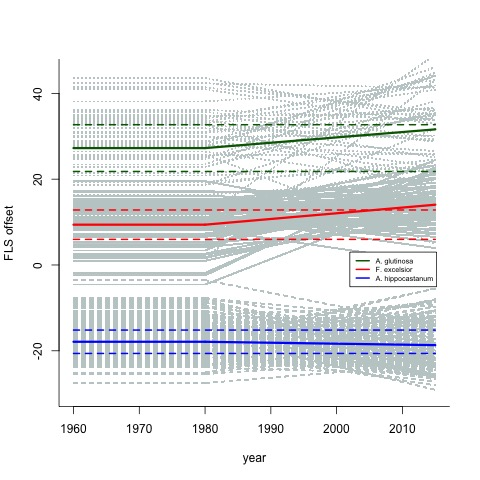
\includegraphics[width=\textwidth]{..//figure/FLS_climate_change.jpeg} 
    \caption{Trends in average FLS offset across Europe for 3 tree species from 1960 to 2015. Dashed lines indicate historic range of FLS variability. All species are increasing their offset, but the rate of change differs between species and and sites}
    \label{fig:Figure 1}
\end{figure}
\begin{figure}
    \centering
    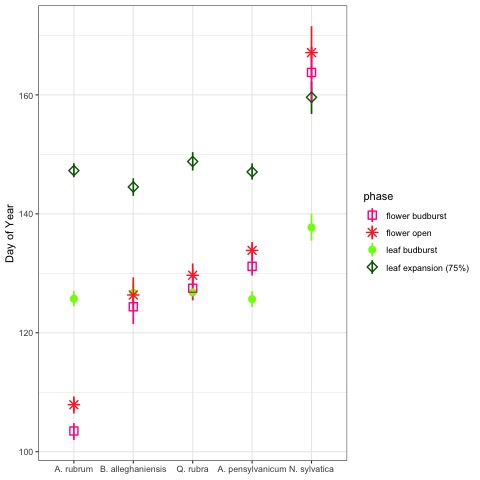
\includegraphics[width=\textwidth]{..//figure/HFmeans.jpeg}
    \caption{Average day of phenological events for highlighted woody plant species at Harvard Forest in Petersham, MA from 1990-2015}
    \label{fig:Figure 2}
\end{figure}
 \begin{figure}
        \centering
          
\includegraphics[width=\textwidth]{..//figure/HF_Q_ru_interannual.jpeg}
        \caption{FLS variability among years and within a population of \textit{Quercus rubra} at Harvard forest.}
        \label{fig: Figure 3}
    \end{figure}
  
    \begin{figure}
    \centering
    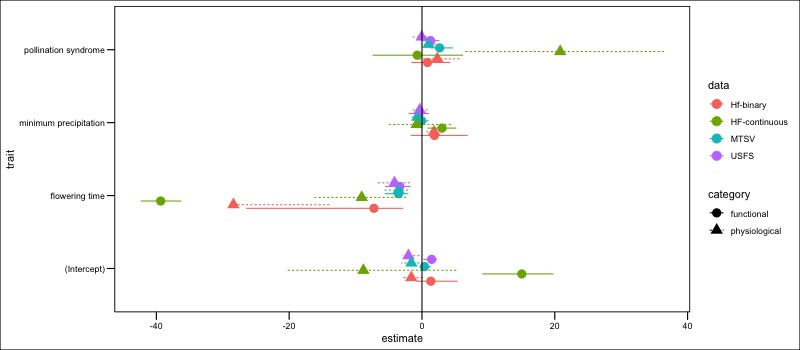
\includegraphics[width=\textwidth]{..//figure/allcases.jpeg}
    \caption{All case study model estimates, phyloglm with 95\% bootstrap intervals}
    \label{fig:Figure 4}
    \end{figure}
    
        \begin{figure}
    \centering
    
\includegraphics[width=\textwidth]{..//figure/cases_2pannel.jpeg}
    \caption{alternatue to figure 4: 4a is phylog glm with 95\% bootstrap intervals, 4b is brms estiamtes with 80\% CIs}
    \label{fig:Figure 5}
    \end{figure}

    
        \begin{figure}[h!]
    \centering
    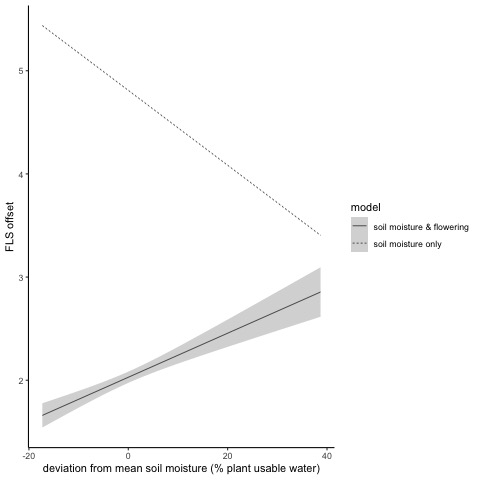
\includegraphics[width=\textwidth]{..//figure/SM_comp.jpeg}
    \caption{effect of soil moisture on FLS offset with (dashed) and without (solid) considering flowering time}
    \label{fig:Figure 6}
    \end{figure}

\pagebreak
\bibliography{..//refs/hyst_outline.bib}

\section*{Supplement}
\subsection*{Methods}
\subsubsection*{Climate Change and FLS:}
To evaluate how FLS patterns have overtime in association with climate change we obtained phenological data for three European woody plant species with long term records of both flower (BBCH 60) and leafout phenology (BBCH 11) from the Pan European Phenological Database \citep{PEP725}. We restricted the data set to include only stations with great than 50 years worth of data. For each species, we modeled FLS offset (day of year leafing- day of year flowering) as a function of time, using a hinge model with 1980 as break point in accordance with climate change models of \citet(). For each species, we displayed the pre-1980 mean and standard devation of FLS offset and the post-1980 change in mean FLS offset that can be associated with climate change.
\subsubsection*{Case studies}
\indent\indent \textbf{MTSV and USFS:} For these two, categorical, species level case studies, we converted verbal descriptions of flower-leaf sequences into a binary response variable. For our more inclusive "functional" definition of hysteranthy, we included species entries with descriptions \textit{"flowers before the leaves"}, \textit{"flowers before or with leaves"} and textit{"flowers with leaves"} as hysteranthous. Our more restrictive "physiological" hysteranthy definition only included species described as \textit{"flowers before the leaves"} as hysteranthous.\\
\ident For modeling trait associates we chose three predictors to represent the three major FLS hypothesis; pollination syndrome, average flowering time and minimum precipitation levels across the species range. Pollination syndrome and average flowering time we obtained directly from the data sources, and estimates of minimum precipitation came from the USDA/NRCS Conservation plants characteristics \citep{}. We coded pollination syndrome as binary, biotic or wind pollinated, with known ambophilous species in the genus \textit{Salix} assigned to the ancestral, biotic pollinated, state of angiosperms. Flowering time was the average of the range of months reported in each data source.\\
\indent \textbf{HF:} For each species in the HF data set, we calculated a continuous mean off FLS "offset" defined here as the average foliate day of the year - average floral day of the year. We approximated our "physiological" FLS characterization be defining offset as (day of leaf budburst-day of flower bud burst) and our "functional" FLS categorization by defining offset as (day of leaf expansion to 75\% of final size- day of first flower open). We also recoded the HF continuous offset variables as continuous with positive offset values coded as hysteranthous and negative values as seranthous.\\
\indent For all species-level case studies (USFS MTSV and HF), associations between hysteranthy and the trait predictors were modeled with logistical regressions in phylogenetic generalized linear modeling framework \citep{Ives2010} using the R package phylolm \citep{Ho2014}.Our models incorporated a published angiosperm phylogenetic tree \citep{Zanne2013} pruned to match the species list for each case study. Species found in the trait data set but not in the original phylogenetic tree were added to the pruned tree at the genus level root. In total 32 species were added to the generic roots for the MTSV data set . We The models were run with 599 bootstrapped re-sampling iterations for each data set \citep{Wilcox2000}. Continuous predictors were re-scaled by subtracting the mean and dividing by two standard deviations to allow for a reasonable comparison of effect sizes between the binary and continuous predictors in this model \citep{Gelman2007}. To assess the phylogenetic structure of hysteranthous flowering, we used the Caper package \citep{Orme2013} to calculate a phylogenetic D statistic.\\
\indent \textbf{PEP 725:} For intra-specific analysis, we utilized phenological records from PEP725 stations in Germany with more than 10 years worth of flowering and leafout records \citep{PEP725} for species \textit{Alnus glutinosa},\textit{Fraxinus excellsior} and \textit {Betula pendula}. To test for associations between FLS variability and inter-annual water availability we modeled the association between FLS and drought years from 2003-2010 using a linear mixed modeling framework with the R package lme4 \citep{Bates2014}. Drought years were determined based on \citet{Ivits_2013}. To test associations for population level variation in FLS and long term soil moisture, we obtained average August soil moisture raster grids 1991-2010 for Germany from the German Weather Service \citep{DWD}, and extracted soil moisture values at every cell. We then tested associations between average soil moisture at each PEP725 phenological station and average FLS for species \textit{Aesculus glabra,} \textit{Alnus glutinosa},\textit{Fraxinus excellsior} and \textit {Betula pendula} using a Bayesian linear mixed model framework with the brms package in R \citep{Burkner2018}. We also repeated the analysis with average April soil moisture data from the same time period and results were robust.\\
\indent Using same PEP725 species records as above, we used linear models to test the relationship between flowering and leaf timing and FLS offset.\\


\begin{figure}[h!]
\begin{tabular}[width=\textwidth]{|c|c|c|}
\hline
Data set&Physiological&Functional\\
\hline
MTSV&0.22&0.07\\
USFS&0.13&0.65\\
HF&0.01&0.27\\
\hline
\end{tabular}
\caption{Phylo.D estimates of phylogentic signal for hysteranthous flowering in three case studies}
\label{fig:Figure S1}
\end{figure}

\begin{figure}[h!]
\begin{tabular}[width=\textwidth]{|c|c|c|c|c|}
\hline
Species&Effect size flowering (sd)&R^2&Effect size leafing (sd)&R^2\\
\hline
Alnus glutinosa&-0.67 (0.002314) &0.58&0.24(0.005)&0.03\\
Fraxinus excellsior&-0.53 (0.002)&0.41&0.24 (0.004)&0.05\\
Aesculus hippocastum& -0.28 (0.002)&0.10&0.411 (0.0019)&0.26 \\
\hline
\end{tabular}
    \caption{Flowering vs leafing influence on hysteranthy}
    \label{fig:Figure S2}
    \end{figure}


\subsection*{Phylogenies}
 \begin{figure}[h!]
    \centering
    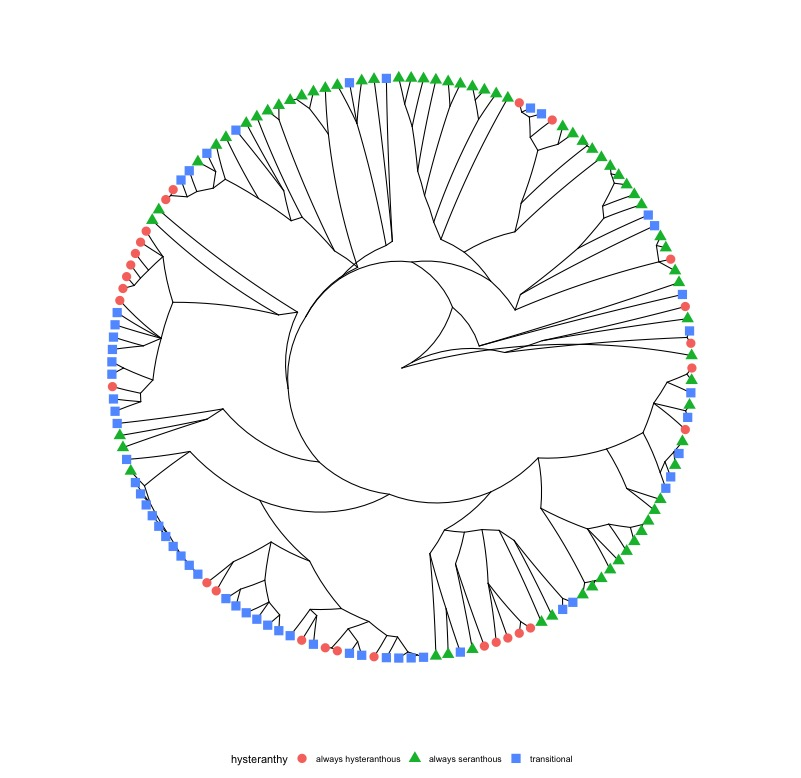
\includegraphics[height=.8\textheight]{..//figure/michtreeplot.jpeg}
    \caption{MTSV phylogeny}
    \label{fig:Figure S3}
    \end{figure}
    
     \begin{figure}
    \centering
    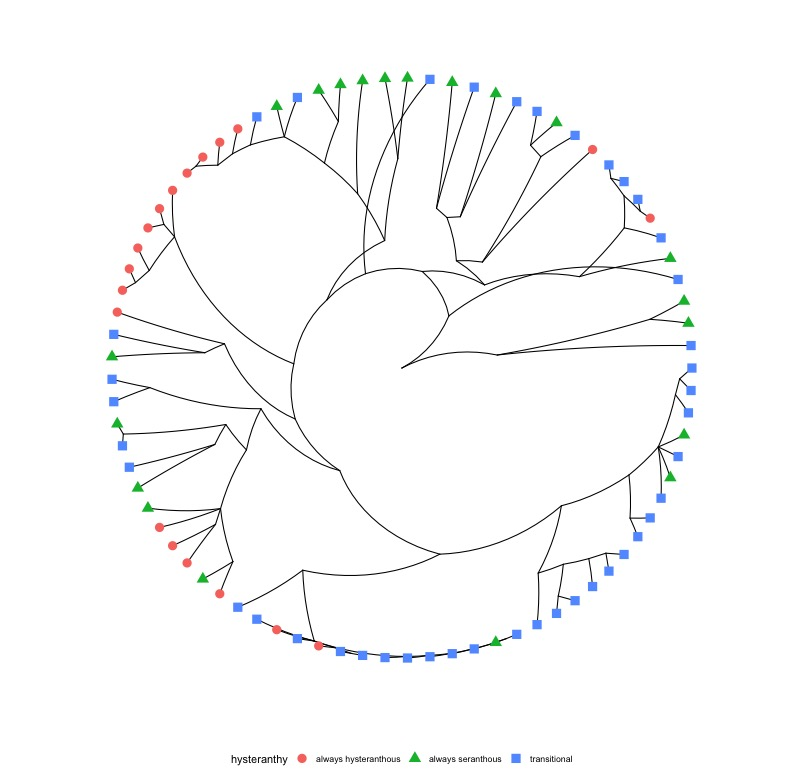
\includegraphics[height=.8\textheight]{..//figure/silvtreeplot.jpeg}
    \caption{USFS Phylogeny}
    \label{fig:Figure S4}
    \end{figure}
    
    \begin{figure}
    \centering
    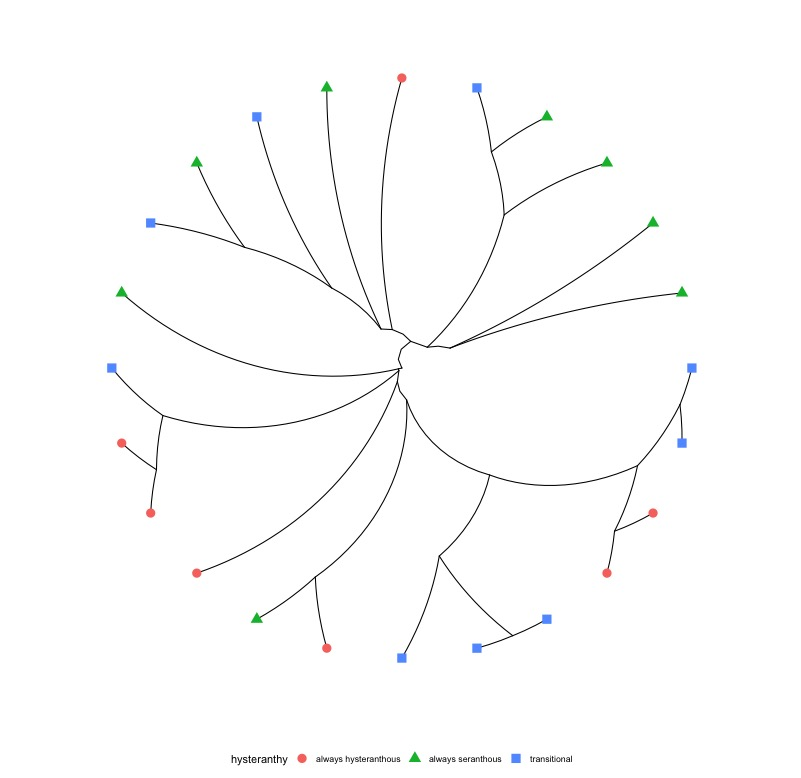
\includegraphics[height=.8\textheight]{..//figure/HFtreeplot.jpeg}
    \caption{HF Phylogeny}
    \label{fig:Figure S5}
    \end{figure}


\end{document}

%Several hypotheses, which will be discussed in more detail in the next section, have been put forward \itepAckerman200,Whitehead1967,Franlkin2006, Janzen1967,Primack1987, Gougherty2018, but direct tests of the fitness benefits of this FLS are rare.
%\section*{Case Studies}
%\indent\indent To further explore the current FLS hypotheses and evaluate how the categorization of FLS and intraspecific variation impact their interpretation, we modeled associations between relevant functional and environmental traits and measures of FLS in four datasets from the temperate northern hemisphere. We will begin by introducing each data set, briefly describing the data structure, modeling choices and inference space for each case. We then compare our resulting models for each case study, considering how these four cases in concert both clarify and complicated the FLS hypotheses at the inter- and intraspecific levels. 
%\subsubsection*{Data set I: Michigan Trees; Michigan Shrubs and Vines (MTSV)}
 %\indent\indent The first data set is complied from two regional guides books, Michigan Trees \citep{Barnes} and Michigan Shrubs and Vines \citep{Barnes}, in which FLS for 194 woody plants species of eastern North America are given through qualitative, verbal descriptions. In organizing these descriptors into FLS categories, We applied two alternate categorization schemes. Our \textit{functional} FLS classification was meant to accommodate a degree of overlap between flowering and the early stages of leaf out as predicted by the wind pollination hypothesis. In this system, FLS descriptions of "flowers before leaves", "flowers before/with leaves" and "flowers with leaves" were classified as the flowering first FLS. Our \textit{physiological} classification restricted any overlap for the flowering-first classification, and only species described as "flowers before leaves" were considered as flowering-first.
% \subsubsection*{Data set II: United States Forest Services Silvics Manual Vol. II (USFS)}
 %\indent\indent The second data set was compiled from the United States Forest Service's Silvics Manual Vol II \citep{}. These data consist of FLS description for 81 woody plant species, including species from both the eastern and western United States. For the USFS data, we applied the same FLS classification scheme as describe above for the MTSV data. Because of the similar structure of these two datasets, we can evaluate the influence of the data source on FLS inference by comparing the respective model results.
 %\subsubsection*{Data set III: Phenology of Woody Species at Harvard Forest since 1990 (HF)}
%\indent\indent A third data set, already addressed briefly in previous sections, comes from long term phenological observations at Harvard Forest in Petersham MA \citep{O'keefe}. For this case study, we calculated a quantitative estimate of FLS, "FLS offset", defined as flowering day of year subtracted from the leafing day of year, for 24 of the deciduous species from the HF data. Positive values of FLS offset indicate a flowering first FLS, while negative values indicate a leafing first strategy.
%The phenology data was recorded at the individual tree level, and can therefore be used to address question of FLS at both intra- and Inter-specific level. With these quantitative FLS estimates, we approximated our FLS classifications from the categorical data by defining "physiological offset" as the difference between flower and leaf budburst day, and "functional FLS offset" as the difference between flower open day and the day on which expanding leaves 75\% of full size. With these data, we also evaluated the effect of qualitatively categorizing FLS at the species level directly by collapsing positive values of average FLS offset to "flowering first" and average negative values to "leafing first", and comparing the results to the quantitative models.
%\subsubsection*{Data set IV:  The Pan European Phenology Project (PEP725)}
%\indent\indent For the final case study, we obtained long term flowering and leafout observations for 3-7 flowering-first species across Europe from the Pan European Phenology Project's database \citep{}. These data are temporally and spatially explicit allowing for us to calculate FLS offset at each site/year. We included any observation stations with more than 10 years worth of both flowering and leafing observations. While the data set is species poor, this criteria allows for a robust evaluation of individual and population level variability in FLS.\\

%\indent\indent We used the MTSV,USFS and HF datasets to model species level FLS trait association. For these models, we chose three predictors relevant to the existing FLS hypotheses; pollination syndrome (wind pollination hypothesis), flowering time (early flowering hypothesis) and minimum precipitation tolerance across a species' range (water dynamic hypothesis). We also measured the phylogenetic structure of categorical FLS, based on a published angiosperm phylogeny \citep{Zanne}(phylogenetic conservatism hypothesis). \\
%\indent Our investigation of FLS in the PEP725 data focused on intraspecific FLS variation. We tested the predictions of the "early flowering" and "water dynamics hypothesis", evaluating how the interannual and population level variability in FLS was affect by environmental parameters average soil moisture, average last frost date, and precipitation.  

%\section*{Aggregated evidence for the FLS hypotheses}
%\begin{enumerate}
%    \item In the following section we will discuss how considering the collective results from our case studies affect our understanding of the hypotheses. We find associations between functional traits hysteranthy that are predicted by several hypotheses suggesting support for them. 
 %   \begin{enumerate}
  %      \item But these data are limited.
   %     \item Variation in this traits at the intraspecific level should have clear fitness consequences.
    %    \item For example given the same levels of ambient pollen, individuals with more hysteranthy should capture more pollen.
     %   \item these kinds of data haven't been collected, but would allow for a more directed evaluation of the hypotheses.
      
    %\end{enumerate}
  %\item  Considering fitness more explicitly into the study of hysteranthy would be a way to better test the predictions, and this will be discussed below
%\end{enumerate} 

. %say this way bettern
%\subsubsection*{Wind pollination hypothesis}
%\begin{enumerate}
%    \item The wind pollination hypothesis predicts that hysteranthy should be associated with the wind pollination syndrome, and that intraspecific variation in FLS should be minimal because pollination syndrome is conserved at the species level. 
 %   \item Our three interspecific variability models generally supported this prediction, although the strength of the association varied depending on the FLS categorization scheme.
 %   \item As predicted, functional hysteranthy generally showed a stronger association with pollination syndrome.
%    \item Intra-specific hysteranthy variability was higher than expected, given the hypotheses.  One of two things could be happening.
 %   \begin{enumerate}
  %     \item As we mentioned there is there is probably a thresh hold below which small leaves don't matter. It could be that the variability never crosses this thresh hold.
   %     \item Considering individual variability, pollination success is actually reduced in years where flower-leaf overlap increases, but the variability is maintained through physiological constraints and balancing selection.
    %\end{enumerate}
    %\item There is a reasonable framework for testing these possibilities. 
%    \begin{enumerate}
 %       \item Study have modeled pollen flow through open vs. closed canopies, but these kinds of studies couldb e performed at higher temporal resolution to capture this effect at various stages of leaf expansion.
  %      \item you could monitor trees over multiple season to see if variation in hysteranthy correlates with variation in pollination success, or directly manipulate hysteranthy in controlled environments.
   % \end{enumerate}
    %\item Even with this general support of the wind pollination hypothesis, there are a nontrivial number of hysteranthous biotically pollinated taxa. Surely, wind pollination can't explain hysteranthy in these species. Exploring trait associations in this taxonomic subset may help clarify the importance of the other hypotheses.  
    %\end{enumerate}

%\subsubsection*{Water dynamics}
%\begin{enumerate}
 %   \item This water dynamics hypothesis suggests that hysteranthous flowering is drought tolerance adaptation. At the species level, it predicts that increased drought tolerance should be associated with hysteranthous flowering. At the intraspecific level, populations growing in drier regions should show more pronounced hysteranthy and even that hysteranthous offset would increase in dry vs. wet years.
  %  \item We found little support for this hypothesis in our analysis.
   % \begin{enumerate}
    %    \item No effect of drought tolerance in any of the the interspecific models specific.
     %   \item At the intraspecific level, we found that drought years were actually associated with reduced hysteranthy due to a delay in flower.
     %   \item There was a week effect of lower soil moisture predicting increased hysteranthy at the population level when considered alone, but this effect flipped directions when other predictors of hysteranthy, such as early flowering were included in the model. Probably need to explain this more.%
    %\end{enumerate}
    %\item This is surprising given that a recent study using a subset of our data found support for this hypothesis. 
%    \begin{enumerate}
 %       \item This could because because the available trait (min P across range) is not a good proxy for drought tolerance.
 %       \item Or, it could be that water in temperate zone isn't usually limited in the spring, and any species level variation due to drought tolerance arose deeper in evolutionary history. If this is the case, more explicitly incorperating biogeopgraphy into our analysis could help us understand this hypothesis.
  %      \item You could also more explicitly test the predictions of this hypothesis, by investigating the intra-specific FLS variation in long term drought experiments.
   % \end{enumerate}
%\end{enumerate}
%\subsubsection*{Early flowering hypothesis}
%\begin{enumerate}
 %   \item This hypothesis predicts that hysteranthy should be associated with the earliest flowering species. At the species level, it would also suggest that there may be associations between hysteranthy and other functional traits associated with early flowering. At the intraspecific level, this hypothesis predicts that years in which flowering occurs early should be associated with increased hysteranthy. Note*, does it make prediction about populations?
  %  \item All of our analyses should strong support for this hypothesis.
   % \item In all three interspecific models, early flowering time was the strongest predictor of hysternathy no matter how hysteranthy was classified. This effect was maintained even we when subset our data to include only generally early flowering species. See supplement.
  %  \item We also found a strong associated between early flowering and hysteranthous offset at the intraspecific level as well.
  %  Early flowering was associated with increase offset, and this relationship was much stronger than the assoication between early leafing and hysteranthy offset (R2 0.5 vs. 0.03).
   % \item This begs the question does hysteranthy actually matter, or can it be lumped in with the general study of evolution of reproductive phenology, because all that really matters is the absolute timing of flowering and hysteanthy is a physiological by product.
%\item We feel because of the evidence of the wind pollination hypothesis and that relies more on the relative timing of flowering vs leaves as opposed to the absolute timing of one or the other, it is too early to abandon the idea that hysteranthy is a trait of its own.
%\end{enumerate}
%\subsubsection*{Phylogeny}
%\begin{enumerate}
 %   \item This hypothesis predicted that interspecific variation in hysteranthy should show strong phylogenetic patterning in lieu of other functional trait associations. There were no clear prediction about intraspecific variation that could be made without a better understanding of the genetic structure of the populations we examined, so for this hypothesis, we restrict our analysis to hysteranthy at the interspecific level.
  %  \item The phylogenetic signal of hysteranthy, as measured by a D statistics when hysteranthy was treated as a categorical trait and by pagaels lambda when hysteranthy was treated continuous, varied significantly between data sources, and depended on how hysteranthy was classfied.
  %  \item This is not surprising.
   % \begin{enumerate}
    %    \item Changing the classification scheme dramatically changed the patterning of the trait along the tree. See supplement.
     %   \item Also it would be expected that except under extremely high phylogenetic structure changing the number and identities of species in the tree would change the inference.
      %  \item Also, several of the hypotheses (wind pollination, early flowering) correspond to traits that have been show to have their own high phylogenetic structure. *Need another sentence about this.
       % \item Overall, the phylogenetic structure of hysteranthy is low-intermediate. *Might need help about how to say something about this that is a bit smarter.
  %  \end{enumerate}
    
%\subsection*{Hysteranthy and global change}
%Above, we recommended that several of the hysteranthy hypotheses could be better tested be relating variability in hysteranthy to explicitly to fitness measures. This approach is also essential in the context of global change. We began this paper by suggesting FLS patterns are changing with global climate change. IF we can better understand the role of this change in overall plant fitness, will better be able to predict the plant communities of the future and implement conservation and natural resource policies accordingly.
%\end{enumerate}
 %\begin{figure}
  %  \centering
   % 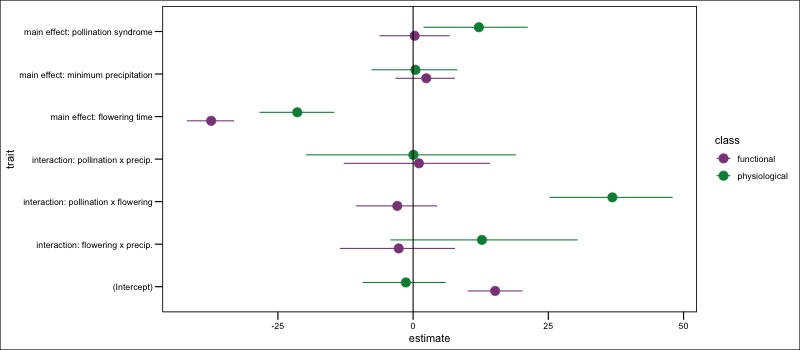
\includegraphics[width=\textwidth]{..//figure/HF_cont_effectsize.jpeg}
    %\caption{Harvard forest continuous . Estimates, 95\% bootstrapping intervals depicted}
    %\label{fig:Figure 6}
    %\end{figure}

